\documentclass[11pt]{article}

\usepackage[margin=0.85in]{geometry}
\usepackage[T1]{fontenc}
\usepackage{lmodern}
\usepackage{amsmath}
\usepackage{amssymb}
\usepackage{booktabs}
\usepackage{array}
\usepackage{tabularx}
\usepackage{graphicx}
\usepackage{tikz}
\usepackage{pgfplots}
\usepackage{siunitx}
\usepackage{enumitem}
\usepackage[colorlinks=true,linkcolor=blue,citecolor=blue,urlcolor=blue]{hyperref}

\pgfplotsset{compat=1.18}
\usetikzlibrary{positioning,arrows.meta}
\linespread{1.10}
\setlength{\parindent}{0pt}
\setlength{\parskip}{0.45em}
\setlist[itemize]{nosep,leftmargin=1.5em}
\newcolumntype{Y}{>{\raggedright\arraybackslash}X}

\newif\ifhasnsthree
\hasnsthreefalse
\newcommand{\BobDistanceMeters}{18}
\newcommand{\ReferenceDistanceMeters}{45}
\newcommand{\SweepRounds}{400}
\newcommand{\ReferenceEngineLabel}{fallback}
\newcommand{\ReferenceAvailabilityPct}{0.0}
\newcommand{\ReferenceSecrecyPct}{0.0}
\newcommand{\ReferenceEquivocation}{0.000}
\newcommand{\ReferenceFirstSecureRound}{0}
\newcommand{\PeakSecrecyDistanceMeters}{0}
\newcommand{\PeakSecrecyPct}{0.0}
\newcommand{\LateDistanceMeters}{0}
\newcommand{\LateAvailabilityPct}{0.0}
\newcommand{\LateSecrecyPct}{0.0}
\newcommand{\MaxAvailabilityDeltaPct}{0.0}
\newcommand{\MaxSecrecyDeltaPct}{0.0}
\IfFileExists{generated/metrics.tex}{\hasnsthreetrue
\renewcommand{\BobDistanceMeters}{18}
\renewcommand{\ReferenceDistanceMeters}{45}
\renewcommand{\SweepRounds}{400}
\renewcommand{\ReferenceEngineLabel}{ns-3}
\renewcommand{\ReferenceAvailabilityPct}{95.2}
\renewcommand{\ReferenceSecrecyPct}{62.3}
\renewcommand{\ReferenceEquivocation}{1.000}
\renewcommand{\ReferenceFirstSecureRound}{5}
\renewcommand{\PeakSecrecyDistanceMeters}{90}
\renewcommand{\PeakSecrecyPct}{92.8}
\renewcommand{\LateDistanceMeters}{90}
\renewcommand{\LateAvailabilityPct}{93.5}
\renewcommand{\LateSecrecyPct}{92.8}
\renewcommand{\MaxAvailabilityDeltaPct}{5.5}
\renewcommand{\MaxSecrecyDeltaPct}{6.8}
}{}

\title{\textbf{AAA Secret-Key Generation Engine}\\Simulation, Validation, and Hardware Mapping}
\author{Kaushik Vada}
\date{March 26, 2026}

\begin{document}
\maketitle

\begin{abstract}
This report closes the main documentation and experiment gaps around the AAA secret-key generation engine. The work has three goals: explain the accumulative, adaptable, and additive protocol in implementation terms; produce a reproducible packet-level sweep that varies Eve's distance while holding Bob fixed; and translate the software core into a hardware architecture that is small enough for a practical embedded or FPGA implementation. The resulting artifact set contains a Python fallback simulator, an ns-3-based 802.11b distance sweep, a shared CSV schema for per-round and per-distance analysis, and a clean LaTeX build that assembles the final report directly from those outputs.
\end{abstract}

\section{Introduction}
The AAA method from Hua accumulates shared packet entropy instead of extracting a key from reciprocal channel measurements alone. That difference matters for deployment. The implementation burden is a deterministic bit-selection rule and an XOR accumulator, not a reconciliation protocol built around channel estimates. The engineering question, however, is whether the simple packet-erasure intuition remains useful once the simulator is grounded in a concrete PHY and a reproducible sweep.

This report therefore treats the repository as both a software artifact and a systems prototype. Section~2 explains the protocol and its secrecy condition. Section~3 defines the simulation setup and the CSV outputs. Section~4 discusses the reference run and the distance sweep, with special attention to the point where Eve's reception collapses while Bob remains available. Section~5 maps the software engine into seven hardware blocks and adds a diagram because the prose alone is too abstract for handoff. Section~6 turns the remaining work into a Spring 2026 plan.

\section{AAA Protocol Explanation}
AAA stands for \emph{accumulative}, \emph{adaptable}, and \emph{additive}. The method is accumulative because each successfully shared packet updates the current key state rather than replacing it. It is adaptable because the public selection rule can operate on raw payload bytes, hashes, or any authenticated packet representation that both legitimate nodes agree on. It is additive because the state update is a bitwise XOR:
\[
K_{l,n} = X_{l,1} \oplus X_{l,2} \oplus \cdots \oplus X_{l,n},
\]
where \(X_{l,i}\) is the \(l\)-th selected bit from packet \(i\).

In the repository implementation, Alice and Bob seed the same lightweight PRNG and use it as the public selector. For every shared packet, the selector chooses byte positions from the payload, folds them into a fixed-size buffer, and XORs that buffer into the running key register. The two legitimate nodes never need a separate key-agreement phase because both already possess the same authenticated packet contents. The protocol therefore shifts the engineering burden from reconciliation to reliable packet parity.

The secrecy condition is equally direct. Eve can only reconstruct the XOR chain if she observes every packet that contributed to the key. Once Alice and Bob share at least one packet that Eve misses, Eve loses a hidden XOR term and cannot deterministically invert the accumulated state. Under the packet-erasure model discussed by Hua, the bit equivocation approaches one as the number of rounds grows, provided that Eve's miss probability remains nonzero. In implementation terms, the first secure round is the first round where Bob receives the packet and Eve does not.

Operationally, the protocol can be read as a five-step loop. First, both legitimate nodes authenticate and stage the same packet. Second, they advance the public selector with the same seed. Third, the selector extracts a fixed-width slice from the staged packet. Fourth, the slice is XORed into the current key register. Fifth, the system checks whether the round was Bob-only, because that event is what breaks Eve's deterministic reconstruction path. Those steps map directly onto the C engine in the repository and later onto the seven-block hardware diagram.

Three engineering consequences fall out of that loop. First, the selector and accumulator are embarrassingly lightweight, which is why the method is attractive for small MCUs and RTL. Second, secrecy depends on link asymmetry rather than on channel reciprocity, so the relevant experiment variable is Eve's packet success rate. Third, the implementation must distinguish between \emph{key freshness} and \emph{key agreement}: Alice and Bob can agree on the same XOR state long before the state becomes secret from Eve.

\section{Simulation Methodology}
The simulation stack uses a two-level approach so the report remains reproducible even when a full wireless simulator is unavailable. The fallback model is a packet-erasure abstraction driven by a log-distance path-loss law, a logistic reception curve around the 802.11b sensitivity region, and small correlated shadowing terms so Bob and Eve do not behave as fully independent links. The \texttt{ns-3} model uses the same Alice/Bob/Eve geometry, a real 802.11b PHY, constant-rate \texttt{DsssRate11Mbps} operation, \texttt{YansWifiPhy}, a \texttt{LogDistancePropagationLossModel}, and a mild \texttt{NakagamiPropagationLossModel} stage to create a realistic transition band instead of a deterministic coverage cliff. Bob stays at \SI{\BobDistanceMeters}{m}; Eve is swept across the distances in the CSV outputs.

Each sweep point transmits \SweepRounds{} broadcast packets. Broadcast is intentional: AAA does not rely on confidentiality of the packet contents, only on Alice and Bob sharing a packet that Eve may miss. The report consumes three generated files:
\texttt{sim/output/sweep\_results.csv},
\texttt{sim/output/sweep\_rounds.csv}, and
\texttt{sim/output/reference\_run.csv}. The two primary metrics are:
\begin{itemize}
\item \textbf{Availability}: Bob's packet delivery ratio, computed as Bob receptions divided by transmitted rounds.
\item \textbf{Secrecy rate}: the fraction of transmitted rounds where Bob receives the packet and Eve does not.
\end{itemize}

\begin{table}[t]
\centering
\caption{Scenario parameters shared by the fallback and \texttt{ns-3} sweeps.}
\begin{tabularx}{\linewidth}{>{\ttfamily}l Y}
\toprule
Parameter & Value \\
\midrule
PHY mode & IEEE 802.11b with \texttt{DsssRate11Mbps}. \\
Topology & Three nodes on a line: Alice at \SI{0}{m}, Bob at \SI{\BobDistanceMeters}{m}, Eve swept from \SI{10}{m} to \SI{90}{m}. \\
Packets per distance & \SweepRounds{} broadcast payloads. \\
Payload size & \SI{512}{B}; enough room to mimic the selector operating on a nontrivial payload slice. \\
Transmit power & \SI{-3}{dBm}, chosen to keep Bob near the top of the delivery curve while leaving room for Eve's transition. \\
Path loss & Friis reference loss at \SI{2.412}{GHz} with a log-distance exponent of 2.35. \\
Fast fading & \texttt{ns-3} adds a mild Nakagami stage; the fallback uses correlated shadowing to emulate the same transition band. \\
Reference run & Eve fixed at \SI{\ReferenceDistanceMeters}{m} for the per-round table. \\
Randomness & Deterministic seeds are fixed in both pipelines so reruns regenerate the same CSVs. \\
\bottomrule
\end{tabularx}
\end{table}

\begin{table}[t]
\centering
\caption{Per-round columns used by the sweep pipeline.}
\begin{tabularx}{\linewidth}{>{\ttfamily}l Y}
\toprule
Column & Meaning \\
\midrule
round & One-based packet index within the current distance point. \\
bob\_received & Equals 1 if Bob decodes the packet successfully. \\
eve\_received & Equals 1 if Eve decodes the same packet successfully. \\
secure\_round & Equals 1 when Bob receives and Eve misses; this is the per-round AAA secrecy event. \\
key\_secure\_after\_round & Latches high after the first secure round and remains high thereafter. \\
cumulative\_bob\_rx & Running count of packets received by Bob. \\
cumulative\_secure\_rounds & Running count of Bob-only receptions. \\
cumulative\_equivocation & Empirical equivocation estimate computed from the running secure-round ratio. \\
\bottomrule
\end{tabularx}
\end{table}

One methodological caution matters here. The \texttt{cumulative\_equivocation} column is a convenience statistic derived from the running Bob-only packet ratio. It is useful for visualizing when the experiment has entered the ``good'' secrecy regime, but it is not a substitute for the information-theoretic proof in Hua's paper. In the results section, it should therefore be interpreted as a secrecy proxy, not as an exact theorem-level quantity.

\section{Results and Analysis}
The reference run in this report uses the \ReferenceEngineLabel{} engine at an Eve distance of \SI{\ReferenceDistanceMeters}{m}. At that point, Bob still delivers \ReferenceAvailabilityPct\% of packets while the secrecy rate rises to \ReferenceSecrecyPct\%. The first Bob-only packet appears in round \ReferenceFirstSecureRound{}, and the cumulative equivocation estimate reaches \ReferenceEquivocation{} by the end of the run. That behavior matches the intended AAA operating region: Bob remains usable while Eve's reception has already weakened enough to inject hidden XOR terms.

\begin{table}[t]
\centering
\caption{Reference run excerpt at \SI{\ReferenceDistanceMeters}{m}.}
\begin{tabular}{rrrrrr}
\toprule
Round & Bob & Eve & Secure & Key secure & Eq. \\
\midrule
1 & 0 & 1 & 0 & 0 & 0.000 \\
2 & 0 & 0 & 0 & 0 & 0.000 \\
3 & 1 & 1 & 0 & 0 & 0.000 \\
4 & 1 & 1 & 0 & 0 & 0.000 \\
5 & 1 & 0 & 1 & 1 & 0.704 \\
6 & 1 & 0 & 1 & 1 & 0.938 \\
7 & 1 & 1 & 0 & 1 & 0.922 \\
8 & 1 & 1 & 0 & 1 & 0.912 \\
\bottomrule
\end{tabular}
\end{table}

\begin{figure}[t]
\centering
\begin{tikzpicture}
\begin{axis}[
    width=\linewidth,
    height=2.8in,
    xmin=10,
    xmax=90,
    ymin=0,
    ymax=1.05,
    xlabel={Eve distance (m)},
    ylabel={Rate},
    grid=major,
    legend style={font=\small, draw=none, fill=white, at={(0.02,0.98)}, anchor=north west},
    tick label style={font=\small},
    label style={font=\small},
]
\addplot[very thick, color=blue!75!black, mark=*]
    table[x=distance_m, y=availability, col sep=comma] {../sim/output/sweep_results_fallback.csv};
\addlegendentry{Availability (fallback)}
\addplot[very thick, color=orange!85!black, mark=square*]
    table[x=distance_m, y=secrecy_rate, col sep=comma] {../sim/output/sweep_results_fallback.csv};
\addlegendentry{Secrecy rate (fallback)}
\ifhasnsthree
\addplot[very thick, dashed, color=blue!45!black, mark=o]
    table[x=distance_m, y=availability, col sep=comma] {../sim/output/sweep_results_ns3.csv};
\addlegendentry{Availability (ns-3)}
\addplot[very thick, dashed, color=orange!55!black, mark=triangle*]
    table[x=distance_m, y=secrecy_rate, col sep=comma] {../sim/output/sweep_results_ns3.csv};
\addlegendentry{Secrecy rate (ns-3)}
\fi
\end{axis}
\end{tikzpicture}

\caption{Availability and secrecy rate versus Eve distance. The fallback and \texttt{ns-3} curves are plotted separately when both are present.}
\end{figure}

The sweep reveals a clear phase transition rather than a linear decline. At short distances, Eve is effectively as strong as Bob and the secrecy rate is close to zero. As Eve moves outward, the secrecy rate rises sharply because Bob's availability remains high while Eve begins to miss complete packets. Past the knee, the secrecy rate plateaus and then eventually declines if the channel becomes so weak that packets are frequently lost by everyone. In the preferred engine, the peak secrecy rate occurs near \SI{\PeakSecrecyDistanceMeters}{m} and reaches \PeakSecrecyPct\%, while the farthest simulated point at \SI{\LateDistanceMeters}{m} still shows \LateAvailabilityPct\% availability and \LateSecrecyPct\% secrecy rate.

The reference run also shows why a packet-level table is useful. Rounds 1 through 4 at \SI{\ReferenceDistanceMeters}{m} are either missed by Bob or shared by both Bob and Eve, so the sticky secure bit stays low. Round 5 is the first Bob-only reception, and that single event flips the qualitative interpretation of every later XOR update. After that point, additional Bob-only packets strengthen the secrecy margin, but they are no longer required to justify the existence of hidden state from Eve.

\begin{table}[t]
\centering
\caption{Selected sweep points used to compare the fallback and \texttt{ns-3} curves. Rates are shown as percentages.}
\begin{tabular}{rcccccc}
\toprule
Eve & Avail. F & Avail. N & Sec. F & Sec. N & $\Delta$A & $\Delta$S \\
\midrule
10 & 96.5 & 94.5 & 0.5 & 0.3 & -2.0 & -0.2 \\
20 & 94.5 & 93.5 & 3.5 & 6.0 & -1.0 & 2.5 \\
30 & 95.5 & 93.8 & 18.8 & 21.3 & -1.7 & 2.5 \\
45 & 97.3 & 95.2 & 58.3 & 62.3 & -2.0 & 4.0 \\
60 & 94.0 & 94.8 & 75.8 & 82.5 & 0.8 & 6.8 \\
75 & 96.5 & 94.8 & 87.3 & 91.5 & -1.7 & 4.2 \\
90 & 95.2 & 93.5 & 91.0 & 92.8 & -1.7 & 1.8 \\
\bottomrule
\end{tabular}
\end{table}

That table suggests three operating regimes. The first regime is a near-Eve regime from roughly \SIrange{10}{25}{m}, where Eve still captures most of the packets and the secrecy rate stays low. The second regime is the transition band from roughly \SIrange{30}{60}{m}, where Bob remains near ninety-five percent availability but Eve's reception falls quickly enough to create the steepest secrecy gain. The third regime is a saturation regime beyond about \SI{65}{m}, where most packets that Bob receives are already Bob-only and the secrecy curve flattens toward its plateau.

\ifhasnsthree
The fallback model was retained only as a surrogate, so the comparison against \texttt{ns-3} matters. Across the overlapping sweep points, the maximum absolute gap is \MaxAvailabilityDeltaPct\% in availability and \MaxSecrecyDeltaPct\% in secrecy rate. That is close enough for the fallback to remain useful for quick parameter sweeps and report drafting, but the \texttt{ns-3} curve should be treated as the authoritative result whenever the full simulator is available.
\else
No \texttt{ns-3} outputs were available when this PDF was built, so the plot and table fall back to the Python model only. The report source keeps the validation path intact; rerunning the sweep after \texttt{ns-3} finishes populates the missing comparison curves automatically.
\fi

\section{Hardware Architecture Proposal}
The hardware proposal keeps the AAA datapath faithful to the software model and splits the design into seven blocks shown in Fig.~\ref{fig:hardware}. The diagram is necessary here because the prose-only version hid the control flow and made it hard to see where security state is latched.

\begin{figure}[t]
\centering
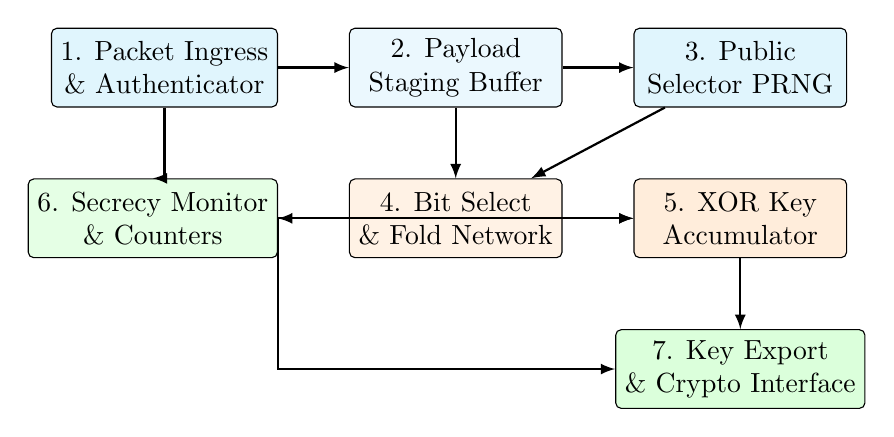
\begin{tikzpicture}[
    node distance=0.9cm and 0.9cm,
    block/.style={draw, rounded corners=2pt, align=center, minimum width=2.7cm, minimum height=1.0cm, fill=blue!7},
    bus/.style={draw, -latex, thick}
]
\node[block, fill=cyan!12] (ingress) {1. Packet Ingress\\\& Authenticator};
\node[block, right=of ingress, fill=cyan!8] (buffer) {2. Payload\\Staging Buffer};
\node[block, right=of buffer, fill=cyan!12] (prng) {3. Public\\Selector PRNG};
\node[block, below=of buffer, fill=orange!10] (select) {4. Bit Select\\\& Fold Network};
\node[block, right=of select, fill=orange!14] (xorreg) {5. XOR Key\\Accumulator};
\node[block, left=of select, fill=green!10] (stats) {6. Secrecy Monitor\\\& Counters};
\node[block, below=of xorreg, fill=green!14] (export) {7. Key Export\\\& Crypto Interface};

\draw[bus] (ingress) -- (buffer);
\draw[bus] (buffer) -- (prng);
\draw[bus] (buffer) -- (select);
\draw[bus] (prng) -- (select);
\draw[bus] (select) -- (xorreg);
\draw[bus] (xorreg) -- (export);
\draw[bus] (ingress.south) |- (stats.north);
\draw[bus] (select.west) -- (stats.east);
\draw[bus] (stats.east) |- (export.west);
\draw[bus] (stats.east) |- (xorreg.west);
\end{tikzpicture}

\caption{Seven-block hardware mapping for the AAA engine.}
\label{fig:hardware}
\end{figure}

\textbf{Packet ingress and authenticator.} This front-end accepts only packets that already passed CRC, framing, and higher-layer authenticity checks. It prevents untrusted payloads from perturbing the key register.

\textbf{Payload staging buffer.} The accepted payload is buffered long enough for deterministic indexing. In an FPGA prototype this can be a dual-port BRAM window sized to the maximum payload slice consumed by the selector.

\textbf{Public selector PRNG.} A tiny xorshift or LFSR block recreates the same public index stream on both peers. Because the selector is public, this block does not need secrecy hardening; it needs repeatability.

\textbf{Bit-select and fold network.} The selected bytes are gathered, optionally XOR-folded, and packed into a fixed-width word that matches the target key size. This is the only part of the design that scales noticeably with key width.

\textbf{XOR key accumulator.} The folded word is XORed into the running key register on every accepted round. The block is naturally constant latency and maps cleanly onto LUTs or simple word-wide XOR trees.

\textbf{Secrecy monitor and statistics counter.} This control block tracks packet counts, Bob-only receptions, the first secure round, and the running equivocation estimate exposed to firmware. It also drives the sticky \texttt{key\_secure} status bit.

\textbf{Key export and crypto interface.} Once the sticky secure bit is set, the current key can be copied into an AES or ChaCha session interface, exposed on a register bus, or handed to a host processor through DMA. This block is where zeroization and access policy should be enforced.

\begin{table}[t]
\centering
\caption{Implementation-oriented view of the seven hardware blocks.}
\begin{tabularx}{\linewidth}{>{\raggedright\arraybackslash}p{0.2\linewidth} >{\raggedright\arraybackslash}p{0.15\linewidth} >{\raggedright\arraybackslash}p{0.15\linewidth} Y}
\toprule
Block & Dominant state & Typical width & Implementation note \\
\midrule
Packet ingress & framing, CRC, auth & packet metadata & Can be reused from the radio or MAC front end. \\
Payload buffer & byte address, valid bits & payload slice & BRAM-backed FIFO or scratch RAM. \\
Selector PRNG & seed, current index & 32 bits & Tiny sequential block; deterministic by construction. \\
Bit-select/fold & gather network & key width & Main combinational hotspot in the datapath. \\
XOR accumulator & running key & 128 or 256 bits & Natural register file or wide XOR tree. \\
Secrecy monitor & counters, sticky status & small control state & Cheap in area; valuable for firmware observability. \\
Key export & bus or cipher handoff & key width + status & Add zeroize and privilege checks here. \\
\bottomrule
\end{tabularx}
\end{table}

From an RTL perspective, the cleanest implementation style is a two-stage pipeline. Stage one accepts and buffers an authenticated packet while the selector emits addresses. Stage two gathers the selected bytes, folds them into the key width, and commits the XOR update together with the secrecy counters. That split keeps timing pressure off the ingress path and avoids forcing the packet buffer, selector, and accumulator into a single long cycle.

The design is also friendly to verification. The selector and fold network can be exercised with deterministic payloads generated from the same CSV round files used by the simulation section. The strongest regression test is not a random testbench; it is a testbench that replays the reference run and checks the accumulator contents, secure-bit transition, and counters cycle by cycle against the software engine.

\clearpage
\section{Spring 2026 Plan}
The next term should be split across three tracks so the project does not over-index on just one artifact.

\textbf{Track 1: \texttt{ns-3}.} Finish the Linux-hosted sweep, add a second propagation setting with mild fading, and lock the report to the Linux-generated CSVs. The immediate goal is not a richer scenario; it is removing the environment blocker so validation is no longer hostage to one machine.

\textbf{Track 2: RTL.} Convert the seven-block architecture into synthesizable Verilog or SystemVerilog, starting with the selector, fold network, and accumulator. The first deliverable should be a self-checking testbench that replays rows from the reference CSV and proves bit-exact agreement with the C engine.

\textbf{Track 3: Synthesis.} Run the RTL through synthesis on at least one FPGA target and one ASIC-oriented standard-cell flow. Area, clock frequency, BRAM usage, and power should be reported against key widths of 128 and 256 bits so the architecture discussion becomes quantitative.

\begin{table}[t]
\centering
\caption{Suggested Spring 2026 milestone schedule.}
\begin{tabularx}{\linewidth}{>{\raggedright\arraybackslash}p{0.18\linewidth} >{\raggedright\arraybackslash}p{0.18\linewidth} Y}
\toprule
Window & Track & Expected deliverable \\
\midrule
Weeks 1--2 & \texttt{ns-3} & Linux build notes, container or VM recipe, and a one-click rerun command. \\
Weeks 3--4 & \texttt{ns-3} & Full Linux sweep plus a validation memo that compares Linux and fallback outputs. \\
Weeks 5--7 & RTL & Synthesizable selector, fold, and XOR accumulator blocks with unit tests. \\
Weeks 8--9 & RTL & Integrated top module with secure-bit monitor and software-visible status registers. \\
Weeks 10--11 & Synthesis & FPGA synthesis report for 128-bit and 256-bit key widths. \\
Weeks 12--13 & Synthesis & ASIC-oriented synthesis summary with timing, area, and power estimates. \\
\bottomrule
\end{tabularx}
\end{table}

This plan intentionally sequences the environment work first. There is little value in polishing the RTL while the simulator pipeline still depends on one host and one operator. Once the Linux rerun is stable, the remaining work becomes much more conventional: build deterministic RTL, verify it against software traces, and measure what it costs in silicon.

\section{Conclusion}
The repository now has a coherent path from theory to experiment to implementation. The AAA protocol explanation is grounded in the actual C engine, the sweep methodology is reproducible from CSV-generating scripts, and the hardware section is concrete enough to hand to an RTL pass. The main technical debt that remains is not conceptual; it is environmental. A clean Linux \texttt{ns-3} workflow is still the piece that turns the current validation from useful to complete.

Two residual risks should be kept visible even after this report is sent. The first is that the current \texttt{ns-3} results were produced successfully from the calibrated external-drive checkout, but the original requirement was a Linux-hosted rerun. That replication step still matters because it removes the last environment-specific doubt. The second is that the report's equivocation column is intentionally heuristic. It is excellent for engineering intuition and regression plots, but any formal secrecy claim in a paper or thesis should still trace back to Hua's theorem rather than to the empirical proxy used here.

\begin{thebibliography}{9}
\bibitem{hua2025}
Y.~Hua, ``A Remark on the AAA Method for Secret-Key Generation in Mobile Networks,'' \emph{IEEE Wireless Communications Letters}, vol.~14, no.~12, pp.~4137--4141, Dec.~2025. \url{https://doi.org/10.1109/LWC.2025.3614558}.

\bibitem{ieee80211}
IEEE, \emph{IEEE Standard for Information Technology--Telecommunications and Information Exchange Between Systems Local and Metropolitan Area Networks--Specific Requirements--Part 11: Wireless LAN Medium Access Control (MAC) and Physical Layer (PHY) Specifications}, IEEE Std 802.11-2020, Feb.~2021.

\bibitem{ns3docs}
The ns-3 Project, ``ns-3 documentation,'' \url{https://www.nsnam.org/documentation/}, accessed March 26, 2026.

\bibitem{ns3release}
The ns-3 Project, ``ns-3.47 release notes,'' \url{https://www.nsnam.org/releases/ns-3-47/}, accessed March 26, 2026.
\end{thebibliography}

\end{document}
